\documentclass[1p]{elsarticle_modified}
%\bibliographystyle{elsarticle-num}

%\usepackage[colorlinks]{hyperref}
%\usepackage{abbrmath_seonhwa} %\Abb, \Ascr, \Acal ,\Abf, \Afrak
\usepackage{amsfonts}
\usepackage{amssymb}
\usepackage{amsmath}
\usepackage{amsthm}
\usepackage{scalefnt}
\usepackage{amsbsy}
\usepackage{kotex}
\usepackage{caption}
\usepackage{subfig}
\usepackage{color}
\usepackage{graphicx}
\usepackage{xcolor} %% white, black, red, green, blue, cyan, magenta, yellow
\usepackage{float}
\usepackage{setspace}
\usepackage{hyperref}

\usepackage{tikz}
\usetikzlibrary{arrows}

\usepackage{multirow}
\usepackage{array} % fixed length table
\usepackage{hhline}

%%%%%%%%%%%%%%%%%%%%%
\makeatletter
\renewcommand*\env@matrix[1][\arraystretch]{%
	\edef\arraystretch{#1}%
	\hskip -\arraycolsep
	\let\@ifnextchar\new@ifnextchar
	\array{*\c@MaxMatrixCols c}}
\makeatother %https://tex.stackexchange.com/questions/14071/how-can-i-increase-the-line-spacing-in-a-matrix
%%%%%%%%%%%%%%%

\usepackage[normalem]{ulem}

\newcommand{\msout}[1]{\ifmmode\text{\sout{\ensuremath{#1}}}\else\sout{#1}\fi}
%SOURCE: \msout is \stkout macro in https://tex.stackexchange.com/questions/20609/strikeout-in-math-mode

\newcommand{\cancel}[1]{
	\ifmmode
	{\color{red}\msout{#1}}
	\else
	{\color{red}\sout{#1}}
	\fi
}

\newcommand{\add}[1]{
	{\color{blue}\uwave{#1}}
}

\newcommand{\replace}[2]{
	\ifmmode
	{\color{red}\msout{#1}}{\color{blue}\uwave{#2}}
	\else
	{\color{red}\sout{#1}}{\color{blue}\uwave{#2}}
	\fi
}

\newcommand{\Sol}{\mathcal{S}} %segment
\newcommand{\D}{D} %diagram
\newcommand{\A}{\mathcal{A}} %arc


%%%%%%%%%%%%%%%%%%%%%%%%%%%%%5 test

\def\sl{\operatorname{\textup{SL}}(2,\Cbb)}
\def\psl{\operatorname{\textup{PSL}}(2,\Cbb)}
\def\quan{\mkern 1mu \triangleright \mkern 1mu}

\theoremstyle{definition}
\newtheorem{thm}{Theorem}[section]
\newtheorem{prop}[thm]{Proposition}
\newtheorem{lem}[thm]{Lemma}
\newtheorem{ques}[thm]{Question}
\newtheorem{cor}[thm]{Corollary}
\newtheorem{defn}[thm]{Definition}
\newtheorem{exam}[thm]{Example}
\newtheorem{rmk}[thm]{Remark}
\newtheorem{alg}[thm]{Algorithm}

\newcommand{\I}{\sqrt{-1}}
\begin{document}

%\begin{frontmatter}
%
%\title{Boundary parabolic representations of knots up to 8 crossings}
%
%%% Group authors per affiliation:
%\author{Yunhi Cho} 
%\address{Department of Mathematics, University of Seoul, Seoul, Korea}
%\ead{yhcho@uos.ac.kr}
%
%
%\author{Seonhwa Kim} %\fnref{s_kim}}
%\address{Center for Geometry and Physics, Institute for Basic Science, Pohang, 37673, Korea}
%\ead{ryeona17@ibs.re.kr}
%
%\author{Hyuk Kim}
%\address{Department of Mathematical Sciences, Seoul National University, Seoul 08826, Korea}
%\ead{hyukkim@snu.ac.kr}
%
%\author{Seokbeom Yoon}
%\address{Department of Mathematical Sciences, Seoul National University, Seoul, 08826,  Korea}
%\ead{sbyoon15@snu.ac.kr}
%
%\begin{abstract}
%We find all boundary parabolic representation of knots up to 8 crossings.
%
%\end{abstract}
%\begin{keyword}
%    \MSC[2010] 57M25 
%\end{keyword}
%
%\end{frontmatter}

%\linenumbers
%\tableofcontents
%
\newcommand\colored[1]{\textcolor{white}{\rule[-0.35ex]{0.8em}{1.4ex}}\kern-0.8em\color{red} #1}%
%\newcommand\colored[1]{\textcolor{white}{ #1}\kern-2.17ex	\textcolor{white}{ #1}\kern-1.81ex	\textcolor{white}{ #1}\kern-2.15ex\color{red}#1	}

{\Large $\underline{12n_{0102}~(K12n_{0102})}$}

\setlength{\tabcolsep}{10pt}
\renewcommand{\arraystretch}{1.6}
\vspace{1cm}\begin{tabular}{m{100pt}>{\centering\arraybackslash}m{274pt}}
\multirow{5}{120pt}{
	\centering
	\includegraphics[width=112pt]{../../../GIT/diagram.site/Diagrams/png/2191_12n_0102.png}\\
\ \ \ A knot diagram\footnotemark}&
\allowdisplaybreaks
\textbf{Linearized knot diagam} \\
\cline{2-2}
 &
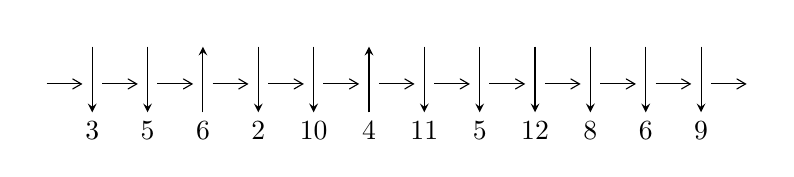
\begin{tikzpicture}[x=20pt, y=17pt]
	% nodes
	\node (C0) at (0, 0) {};
	\node (C1) at (1, 0) {};
	\node (C1U) at (1, +1) {};
	\node (C1D) at (1, -1) {3};

	\node (C2) at (2, 0) {};
	\node (C2U) at (2, +1) {};
	\node (C2D) at (2, -1) {5};

	\node (C3) at (3, 0) {};
	\node (C3U) at (3, +1) {};
	\node (C3D) at (3, -1) {6};

	\node (C4) at (4, 0) {};
	\node (C4U) at (4, +1) {};
	\node (C4D) at (4, -1) {2};

	\node (C5) at (5, 0) {};
	\node (C5U) at (5, +1) {};
	\node (C5D) at (5, -1) {10};

	\node (C6) at (6, 0) {};
	\node (C6U) at (6, +1) {};
	\node (C6D) at (6, -1) {4};

	\node (C7) at (7, 0) {};
	\node (C7U) at (7, +1) {};
	\node (C7D) at (7, -1) {11};

	\node (C8) at (8, 0) {};
	\node (C8U) at (8, +1) {};
	\node (C8D) at (8, -1) {5};

	\node (C9) at (9, 0) {};
	\node (C9U) at (9, +1) {};
	\node (C9D) at (9, -1) {12};

	\node (C10) at (10, 0) {};
	\node (C10U) at (10, +1) {};
	\node (C10D) at (10, -1) {8};

	\node (C11) at (11, 0) {};
	\node (C11U) at (11, +1) {};
	\node (C11D) at (11, -1) {6};

	\node (C12) at (12, 0) {};
	\node (C12U) at (12, +1) {};
	\node (C12D) at (12, -1) {9};
	\node (C13) at (13, 0) {};

	% arrows
	\draw[->,>={angle 60}]
	(C0) edge (C1) (C1) edge (C2) (C2) edge (C3) (C3) edge (C4) (C4) edge (C5) (C5) edge (C6) (C6) edge (C7) (C7) edge (C8) (C8) edge (C9) (C9) edge (C10) (C10) edge (C11) (C11) edge (C12) (C12) edge (C13) ;	\draw[->,>=stealth]
	(C1U) edge (C1D) (C2U) edge (C2D) (C3D) edge (C3U) (C4U) edge (C4D) (C5U) edge (C5D) (C6D) edge (C6U) (C7U) edge (C7D) (C8U) edge (C8D) (C9U) edge (C9D) (C10U) edge (C10D) (C11U) edge (C11D) (C12U) edge (C12D) ;
	\end{tikzpicture} \\
\hhline{~~} \\& 
\textbf{Solving Sequence} \\ \cline{2-2} 
 &
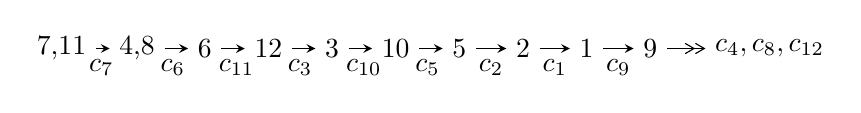
\begin{tikzpicture}[x=23pt, y=7pt]
	% node
	\node (A0) at (-1/8, 0) {7,11};
	\node (A1) at (17/16, 0) {4,8};
	\node (A2) at (17/8, 0) {6};
	\node (A3) at (25/8, 0) {12};
	\node (A4) at (33/8, 0) {3};
	\node (A5) at (41/8, 0) {10};
	\node (A6) at (49/8, 0) {5};
	\node (A7) at (57/8, 0) {2};
	\node (A8) at (65/8, 0) {1};
	\node (A9) at (73/8, 0) {9};
	\node (C1) at (1/2, -1) {$c_{7}$};
	\node (C2) at (13/8, -1) {$c_{6}$};
	\node (C3) at (21/8, -1) {$c_{11}$};
	\node (C4) at (29/8, -1) {$c_{3}$};
	\node (C5) at (37/8, -1) {$c_{10}$};
	\node (C6) at (45/8, -1) {$c_{5}$};
	\node (C7) at (53/8, -1) {$c_{2}$};
	\node (C8) at (61/8, -1) {$c_{1}$};
	\node (C9) at (69/8, -1) {$c_{9}$};
	\node (A10) at (11, 0) {$c_{4},c_{8},c_{12}$};

	% edge
	\draw[->,>=stealth]	
	(A0) edge (A1) (A1) edge (A2) (A2) edge (A3) (A3) edge (A4) (A4) edge (A5) (A5) edge (A6) (A6) edge (A7) (A7) edge (A8) (A8) edge (A9) ;
	\draw[->>,>={angle 60}]	
	(A9) edge (A10);
\end{tikzpicture} \\ 

\end{tabular} \\

\footnotetext{
The image of knot diagram is generated by the software ``\textbf{Draw programme}" developed by Andrew Bartholomew(\url{http://www.layer8.co.uk/maths/draw/index.htm\#Running-draw}), where we modified some parts for our purpose(\url{https://github.com/CATsTAILs/LinksPainter}).
}\phantom \\ \newline 
\centering \textbf{Ideals for irreducible components\footnotemark of $X_{\text{par}}$} 
 
\begin{align*}
I^u_{1}&=\langle 
8320485 u^{18}+10563177 u^{17}+\cdots+38476288 b-13934311,\\
\phantom{I^u_{1}}&\phantom{= \langle  }577476311 u^{18}+1351379411 u^{17}+\cdots+615620608 a-4237296637,\;u^{19}+2 u^{18}+\cdots-7 u+1\rangle \\
I^u_{2}&=\langle 
6839 a^5 u+100530 a^4 u+\cdots-679911 a+101996,\\
\phantom{I^u_{2}}&\phantom{= \langle  }a^6+5 a^5 u-6 a^5-20 a^4 u+2 a^4+16 a^3 u+22 a^3+6 a^2 u-29 a^2-8 a u+7 a+u,\;u^2+1\rangle \\
I^u_{3}&=\langle 
b,\;5 u^2+4 a+3 u+11,\;u^3+2 u-1\rangle \\
I^u_{4}&=\langle 
-4214 u^9-17396 u^8+\cdots+334809 b-381952,\\
\phantom{I^u_{4}}&\phantom{= \langle  }-40716 u^9+776951 u^8+\cdots+5691753 a-2589163,\\
\phantom{I^u_{4}}&\phantom{= \langle  }u^{10}- u^8+15 u^6- u^5+57 u^4+7 u^3+56 u^2+12 u+17\rangle \\
I^u_{5}&=\langle 
b,\;u^3+a+u,\;u^4+u^3+2 u^2+2 u+1\rangle \\
\\
\end{align*}
\raggedright * 5 irreducible components of $\dim_{\mathbb{C}}=0$, with total 48 representations.\\
\footnotetext{All coefficients of polynomials are rational numbers. But the coefficients are sometimes approximated in decimal forms when there is not enough margin.}
\newpage
\renewcommand{\arraystretch}{1}
\centering \section*{I. $I^u_{1}= \langle 8.32\times10^{6} u^{18}+1.06\times10^{7} u^{17}+\cdots+3.85\times10^{7} b-1.39\times10^{7},\;5.77\times10^{8} u^{18}+1.35\times10^{9} u^{17}+\cdots+6.16\times10^{8} a-4.24\times10^{9},\;u^{19}+2 u^{18}+\cdots-7 u+1 \rangle$}
\flushleft \textbf{(i) Arc colorings}\\
\begin{tabular}{m{7pt} m{180pt} m{7pt} m{180pt} }
\flushright $a_{7}=$&$\begin{pmatrix}1\\0\end{pmatrix}$ \\
\flushright $a_{11}=$&$\begin{pmatrix}0\\u\end{pmatrix}$ \\
\flushright $a_{4}=$&$\begin{pmatrix}-0.938039 u^{18}-2.19515 u^{17}+\cdots-14.3029 u+6.88297\\-0.216250 u^{18}-0.274537 u^{17}+\cdots-5.00433 u+0.362153\end{pmatrix}$ \\
\flushright $a_{8}=$&$\begin{pmatrix}1\\u^2\end{pmatrix}$ \\
\flushright $a_{6}=$&$\begin{pmatrix}0.628575 u^{18}+1.63591 u^{17}+\cdots-1.38123 u-0.584679\\-0.299899 u^{18}-0.718244 u^{17}+\cdots+0.505642 u-0.218705\end{pmatrix}$ \\
\flushright $a_{12}=$&$\begin{pmatrix}0.00390625 u^{18}+0.00390625 u^{17}+\cdots+1.96875 u-0.996094\\0.00781250 u^{18}+0.00781250 u^{17}+\cdots+1.93750 u+0.00781250\end{pmatrix}$ \\
\flushright $a_{3}=$&$\begin{pmatrix}-0.437270 u^{18}-1.23881 u^{17}+\cdots-4.63744 u+5.33139\\0.000159761 u^{18}+0.202746 u^{17}+\cdots-8.42258 u+0.956342\end{pmatrix}$ \\
\flushright $a_{10}=$&$\begin{pmatrix}u\\u^3+u\end{pmatrix}$ \\
\flushright $a_{5}=$&$\begin{pmatrix}0.602641 u^{18}+1.62088 u^{17}+\cdots-3.67950 u-0.116155\\-0.324143 u^{18}-0.736442 u^{17}+\cdots-1.50878 u+0.212974\end{pmatrix}$ \\
\flushright $a_{2}=$&$\begin{pmatrix}-1.35943 u^{18}-3.14988 u^{17}+\cdots-11.6390 u+6.93843\\0.201483 u^{18}+0.509159 u^{17}+\cdots-3.35421 u+0.130337\end{pmatrix}$ \\
\flushright $a_{1}=$&$\begin{pmatrix}-0.00781250 u^{18}-0.00781250 u^{17}+\cdots-1.93750 u+0.992188\\-0.0156250 u^{18}-0.0156250 u^{17}+\cdots-1.87500 u-0.0156250\end{pmatrix}$ \\
\flushright $a_{9}=$&$\begin{pmatrix}0.00390625 u^{18}+0.00390625 u^{17}+\cdots+1.96875 u+0.00390625\\0.00781250 u^{18}+0.00781250 u^{17}+\cdots+0.937500 u+0.00781250\end{pmatrix}$\\&\end{tabular}
\flushleft \textbf{(ii) Obstruction class $= -1$}\\~\\
\flushleft \textbf{(iii) Cusp Shapes $= -\frac{9530088851}{2462482432} u^{18}-\frac{22393935231}{2462482432} u^{17}+\cdots-\frac{7325733887}{615620608} u+\frac{3696058001}{2462482432}$}\\~\\
\newpage\renewcommand{\arraystretch}{1}
\flushleft \textbf{(iv) u-Polynomials at the component}\newline \\
\begin{tabular}{m{50pt}|m{274pt}}
Crossings & \hspace{64pt}u-Polynomials at each crossing \\
\hline $$\begin{aligned}c_{1}\end{aligned}$$&$\begin{aligned}
&u^{19}+18 u^{18}+\cdots+45729 u+256
\end{aligned}$\\
\hline $$\begin{aligned}c_{2},c_{4}\end{aligned}$$&$\begin{aligned}
&u^{19}-4 u^{18}+\cdots+225 u-16
\end{aligned}$\\
\hline $$\begin{aligned}c_{3},c_{6}\end{aligned}$$&$\begin{aligned}
&u^{19}+3 u^{18}+\cdots+688 u+128
\end{aligned}$\\
\hline $$\begin{aligned}c_{5}\end{aligned}$$&$\begin{aligned}
&u^{19}-6 u^{18}+\cdots+12 u-4
\end{aligned}$\\
\hline $$\begin{aligned}c_{7},c_{9},c_{10}\\c_{12}\end{aligned}$$&$\begin{aligned}
&u^{19}-2 u^{18}+\cdots-7 u-1
\end{aligned}$\\
\hline $$\begin{aligned}c_{8},c_{11}\end{aligned}$$&$\begin{aligned}
&u^{19}-29 u^{17}+\cdots-320 u+64
\end{aligned}$\\
\hline
\end{tabular}\\~\\
\newpage\renewcommand{\arraystretch}{1}
\flushleft \textbf{(v) Riley Polynomials at the component}\newline \\
\begin{tabular}{m{50pt}|m{274pt}}
Crossings & \hspace{64pt}Riley Polynomials at each crossing \\
\hline $$\begin{aligned}c_{1}\end{aligned}$$&$\begin{aligned}
&y^{19}-46 y^{18}+\cdots+1968323393 y-65536
\end{aligned}$\\
\hline $$\begin{aligned}c_{2},c_{4}\end{aligned}$$&$\begin{aligned}
&y^{19}-18 y^{18}+\cdots+45729 y-256
\end{aligned}$\\
\hline $$\begin{aligned}c_{3},c_{6}\end{aligned}$$&$\begin{aligned}
&y^{19}+9 y^{18}+\cdots+214272 y-16384
\end{aligned}$\\
\hline $$\begin{aligned}c_{5}\end{aligned}$$&$\begin{aligned}
&y^{19}-2 y^{18}+\cdots+152 y-16
\end{aligned}$\\
\hline $$\begin{aligned}c_{7},c_{9},c_{10}\\c_{12}\end{aligned}$$&$\begin{aligned}
&y^{19}+2 y^{18}+\cdots- y-1
\end{aligned}$\\
\hline $$\begin{aligned}c_{8},c_{11}\end{aligned}$$&$\begin{aligned}
&y^{19}-58 y^{18}+\cdots+106496 y-4096
\end{aligned}$\\
\hline
\end{tabular}\\~\\
\newpage\flushleft \textbf{(vi) Complex Volumes and Cusp Shapes}
$$\begin{array}{c|c|c}  
\text{Solutions to }I^u_{1}& \I (\text{vol} + \sqrt{-1}CS) & \text{Cusp shape}\\
 \hline 
\begin{aligned}
u &= \phantom{-}0.065994 + 0.703453 I \\
a &= \phantom{-}1.146140 - 0.182747 I \\
b &= -1.168000 + 0.494902 I\end{aligned}
 & \phantom{-}2.15420 - 5.93819 I & -10.00409 + 7.04982 I \\ \hline\begin{aligned}
u &= \phantom{-}0.065994 - 0.703453 I \\
a &= \phantom{-}1.146140 + 0.182747 I \\
b &= -1.168000 - 0.494902 I\end{aligned}
 & \phantom{-}2.15420 + 5.93819 I & -10.00409 - 7.04982 I \\ \hline\begin{aligned}
u &= \phantom{-}1.308400 + 0.398474 I \\
a &= \phantom{-}0.207847 + 1.170010 I \\
b &= \phantom{-}0.312558 + 1.138020 I\end{aligned}
 & -3.47657 - 1.31737 I & -6.24812 - 2.66398 I \\ \hline\begin{aligned}
u &= \phantom{-}1.308400 - 0.398474 I \\
a &= \phantom{-}0.207847 - 1.170010 I \\
b &= \phantom{-}0.312558 - 1.138020 I\end{aligned}
 & -3.47657 + 1.31737 I & -6.24812 + 2.66398 I \\ \hline\begin{aligned}
u &= -0.072468 + 0.615756 I \\
a &= -1.048370 + 0.662466 I \\
b &= \phantom{-}1.211950 - 0.244182 I\end{aligned}
 & \phantom{-}3.66948 - 0.63571 I & -5.45626 - 0.87908 I \\ \hline\begin{aligned}
u &= -0.072468 - 0.615756 I \\
a &= -1.048370 - 0.662466 I \\
b &= \phantom{-}1.211950 + 0.244182 I\end{aligned}
 & \phantom{-}3.66948 + 0.63571 I & -5.45626 + 0.87908 I \\ \hline\begin{aligned}
u &= \phantom{-}0.531110\phantom{ +0.000000I} \\
a &= \phantom{-}0.510168\phantom{ +0.000000I} \\
b &= -0.274813\phantom{ +0.000000I}\end{aligned}
 & -0.869373\phantom{ +0.000000I} & -11.1210\phantom{ +0.000000I} \\ \hline\begin{aligned}
u &= -0.27618 + 1.56855 I \\
a &= \phantom{-}0.0759776 + 0.1041410 I \\
b &= \phantom{-}0.191656 - 0.770544 I\end{aligned}
 & \phantom{-}7.41380 + 4.96650 I & -10.42447 + 0.17242 I \\ \hline\begin{aligned}
u &= -0.27618 - 1.56855 I \\
a &= \phantom{-}0.0759776 - 0.1041410 I \\
b &= \phantom{-}0.191656 + 0.770544 I\end{aligned}
 & \phantom{-}7.41380 - 4.96650 I & -10.42447 - 0.17242 I \\ \hline\begin{aligned}
u &= \phantom{-}0.087202 + 0.342519 I \\
a &= \phantom{-}1.53123 + 0.07499 I \\
b &= -0.140322 - 0.778902 I\end{aligned}
 & -0.99829 - 1.27054 I & -8.20061 + 4.97839 I\\
 \hline 
 \end{array}$$\newpage$$\begin{array}{c|c|c}  
\text{Solutions to }I^u_{1}& \I (\text{vol} + \sqrt{-1}CS) & \text{Cusp shape}\\
 \hline 
\begin{aligned}
u &= \phantom{-}0.087202 - 0.342519 I \\
a &= \phantom{-}1.53123 - 0.07499 I \\
b &= -0.140322 + 0.778902 I\end{aligned}
 & -0.99829 + 1.27054 I & -8.20061 - 4.97839 I \\ \hline\begin{aligned}
u &= -1.54056 + 0.78681 I \\
a &= -0.421033 + 1.025860 I \\
b &= \phantom{-}0.73485 + 2.99107 I\end{aligned}
 & -5.13904 + 5.65628 I & -9.07225 - 4.94267 I \\ \hline\begin{aligned}
u &= -1.54056 - 0.78681 I \\
a &= -0.421033 - 1.025860 I \\
b &= \phantom{-}0.73485 - 2.99107 I\end{aligned}
 & -5.13904 - 5.65628 I & -9.07225 + 4.94267 I \\ \hline\begin{aligned}
u &= \phantom{-}0.234786\phantom{ +0.000000I} \\
a &= \phantom{-}6.08809\phantom{ +0.000000I} \\
b &= -0.438368\phantom{ +0.000000I}\end{aligned}
 & -2.17097\phantom{ +0.000000I} & \phantom{-}4.15310\phantom{ +0.000000I} \\ \hline\begin{aligned}
u &= -1.03991 + 1.54219 I \\
a &= \phantom{-}0.810661 - 0.834761 I \\
b &= -1.49692 - 1.76255 I\end{aligned}
 & -12.3003 + 14.4824 I & -6.92108 - 6.18391 I \\ \hline\begin{aligned}
u &= -1.03991 - 1.54219 I \\
a &= \phantom{-}0.810661 + 0.834761 I \\
b &= -1.49692 + 1.76255 I\end{aligned}
 & -12.3003 - 14.4824 I & -6.92108 + 6.18391 I \\ \hline\begin{aligned}
u &= -1.86882\phantom{ +0.000000I} \\
a &= -0.500182\phantom{ +0.000000I} \\
b &= -3.63345\phantom{ +0.000000I}\end{aligned}
 & -8.22250\phantom{ +0.000000I} & -12.0580\phantom{ +0.000000I} \\ \hline\begin{aligned}
u &= \phantom{-}1.01897 + 1.61412 I \\
a &= -0.726491 - 0.564033 I \\
b &= \phantom{-}1.02754 - 1.79037 I\end{aligned}
 & -12.01080 - 6.53502 I & -7.12923 + 2.43738 I \\ \hline\begin{aligned}
u &= \phantom{-}1.01897 - 1.61412 I \\
a &= -0.726491 + 0.564033 I \\
b &= \phantom{-}1.02754 + 1.79037 I\end{aligned}
 & -12.01080 + 6.53502 I & -7.12923 - 2.43738 I\\
 \hline 
 \end{array}$$\newpage\newpage\renewcommand{\arraystretch}{1}
\centering \section*{II. $I^u_{2}= \langle 6839 a^{5} u+1.01\times10^{5} a^{4} u+\cdots-6.80\times10^{5} a+1.02\times10^{5},\;5 a^5 u-20 a^4 u+\cdots-29 a^2+7 a,\;u^2+1 \rangle$}
\flushleft \textbf{(i) Arc colorings}\\
\begin{tabular}{m{7pt} m{180pt} m{7pt} m{180pt} }
\flushright $a_{7}=$&$\begin{pmatrix}1\\0\end{pmatrix}$ \\
\flushright $a_{11}=$&$\begin{pmatrix}0\\u\end{pmatrix}$ \\
\flushright $a_{4}=$&$\begin{pmatrix}a\\-0.163327 a^{5} u-2.40083 a^{4} u+\cdots+16.2375 a-2.43584\end{pmatrix}$ \\
\flushright $a_{8}=$&$\begin{pmatrix}1\\-1\end{pmatrix}$ \\
\flushright $a_{6}=$&$\begin{pmatrix}0.0197263 a^{5} u-0.856399 a^{4} u+\cdots+3.63150 a+0.836673\\-0.0806247 a^{5} u+0.463927 a^{4} u+\cdots-1.15007 a+0.616698\end{pmatrix}$ \\
\flushright $a_{12}=$&$\begin{pmatrix}0.476488 a^{5} u-1.95505 a^{4} u+\cdots-5.95668 a+1.47857\\-1\end{pmatrix}$ \\
\flushright $a_{3}=$&$\begin{pmatrix}0.0829652 a^{5} u+3.40057 a^{4} u+\cdots-16.6394 a+2.51647\\-0.546629 a^{5} u+2.89361 a^{4} u+\cdots+3.20882 a-2.34698\end{pmatrix}$ \\
\flushright $a_{10}=$&$\begin{pmatrix}u\\0\end{pmatrix}$ \\
\flushright $a_{5}=$&$\begin{pmatrix}0.100351 a^{5} u-1.32033 a^{4} u+\cdots+4.78158 a+0.219975\\-0.0806247 a^{5} u+0.463927 a^{4} u+\cdots-1.15007 a+0.616698\end{pmatrix}$ \\
\flushright $a_{2}=$&$\begin{pmatrix}0.121486 a^{5} u+0.333532 a^{4} u+\cdots-4.75610 a+1.54498\\-0.186540 a^{5} u+2.61663 a^{4} u+\cdots-7.68727 a+0.569914\end{pmatrix}$ \\
\flushright $a_{1}=$&$\begin{pmatrix}-1\\0\end{pmatrix}$ \\
\flushright $a_{9}=$&$\begin{pmatrix}0.113677 a^{5} u-2.86738 a^{4} u+\cdots+7.36799 a+0.753708\\- u\end{pmatrix}$\\&\end{tabular}
\flushleft \textbf{(ii) Obstruction class $= 1$}\\~\\
\flushleft \textbf{(iii) Cusp Shapes $= \frac{6556}{41873} a^5 u-\frac{362488}{41873} a^4 u+\cdots+\frac{1586112}{41873} a-\frac{146544}{41873}$}\\~\\
\newpage\renewcommand{\arraystretch}{1}
\flushleft \textbf{(iv) u-Polynomials at the component}\newline \\
\begin{tabular}{m{50pt}|m{274pt}}
Crossings & \hspace{64pt}u-Polynomials at each crossing \\
\hline $$\begin{aligned}c_{1}\end{aligned}$$&$\begin{aligned}
&(u^6-3 u^5+5 u^4-4 u^3+2 u^2- u+1)^2
\end{aligned}$\\
\hline $$\begin{aligned}c_{2},c_{6}\end{aligned}$$&$\begin{aligned}
&(u^6+u^5- u^4-2 u^3+u+1)^2
\end{aligned}$\\
\hline $$\begin{aligned}c_{3},c_{4}\end{aligned}$$&$\begin{aligned}
&(u^6- u^5- u^4+2 u^3- u+1)^2
\end{aligned}$\\
\hline $$\begin{aligned}c_{5}\end{aligned}$$&$\begin{aligned}
&u^{12}- u^{10}+5 u^8+6 u^4-3 u^2+1
\end{aligned}$\\
\hline $$\begin{aligned}c_{7},c_{9},c_{10}\\c_{12}\end{aligned}$$&$\begin{aligned}
&(u^2+1)^6
\end{aligned}$\\
\hline $$\begin{aligned}c_{8}\end{aligned}$$&$\begin{aligned}
&u^{12}-2 u^{11}+\cdots-192 u+64
\end{aligned}$\\
\hline $$\begin{aligned}c_{11}\end{aligned}$$&$\begin{aligned}
&u^{12}+2 u^{11}+\cdots+192 u+64
\end{aligned}$\\
\hline
\end{tabular}\\~\\
\newpage\renewcommand{\arraystretch}{1}
\flushleft \textbf{(v) Riley Polynomials at the component}\newline \\
\begin{tabular}{m{50pt}|m{274pt}}
Crossings & \hspace{64pt}Riley Polynomials at each crossing \\
\hline $$\begin{aligned}c_{1}\end{aligned}$$&$\begin{aligned}
&(y^6+y^5+5 y^4+6 y^2+3 y+1)^2
\end{aligned}$\\
\hline $$\begin{aligned}c_{2},c_{3},c_{4}\\c_{6}\end{aligned}$$&$\begin{aligned}
&(y^6-3 y^5+5 y^4-4 y^3+2 y^2- y+1)^2
\end{aligned}$\\
\hline $$\begin{aligned}c_{5}\end{aligned}$$&$\begin{aligned}
&(y^6- y^5+5 y^4+6 y^2-3 y+1)^2
\end{aligned}$\\
\hline $$\begin{aligned}c_{7},c_{9},c_{10}\\c_{12}\end{aligned}$$&$\begin{aligned}
&(y+1)^{12}
\end{aligned}$\\
\hline $$\begin{aligned}c_{8},c_{11}\end{aligned}$$&$\begin{aligned}
&y^{12}-12 y^{10}+736 y^8-3584 y^6+9472 y^4-9216 y^2+4096
\end{aligned}$\\
\hline
\end{tabular}\\~\\
\newpage\flushleft \textbf{(vi) Complex Volumes and Cusp Shapes}
$$\begin{array}{c|c|c}  
\text{Solutions to }I^u_{2}& \I (\text{vol} + \sqrt{-1}CS) & \text{Cusp shape}\\
 \hline 
\begin{aligned}
u &= \phantom{-0.000000 -}1.000000 I \\
a &= \phantom{-}1.217590 + 0.251449 I \\
b &= -1.073950 - 0.558752 I\end{aligned}
 & \phantom{-}3.28987 + 5.69302 I & -2.00000 - 5.51057 I \\ \hline\begin{aligned}
u &= \phantom{-0.000000 -}1.000000 I \\
a &= -1.010760 - 0.965580 I \\
b &= \phantom{-}1.002190 + 0.295542 I\end{aligned}
 & \phantom{-}5.18047 + 0.92430 I & \phantom{-}1.71672 - 0.79423 I \\ \hline\begin{aligned}
u &= \phantom{-0.000000 -}1.000000 I \\
a &= \phantom{-}0.318306 - 0.177934 I \\
b &= \phantom{-}1.002190 - 0.295542 I\end{aligned}
 & \phantom{-}5.18047 - 0.92430 I & \phantom{-}1.71672 + 0.79423 I \\ \hline\begin{aligned}
u &= \phantom{-0.000000 -}1.000000 I \\
a &= \phantom{-}0.100084 - 0.103550 I \\
b &= -1.073950 + 0.558752 I\end{aligned}
 & \phantom{-}3.28987 - 5.69302 I & -2.00000 + 5.51057 I \\ \hline\begin{aligned}
u &= \phantom{-0.000000 -}1.000000 I \\
a &= \phantom{-}2.39185 - 1.23447 I \\
b &= -0.428243 + 0.664531 I\end{aligned}
 & \phantom{-}1.39926 + 0.92430 I & -5.71672 - 0.79423 I \\ \hline\begin{aligned}
u &= \phantom{-0.000000 -}1.000000 I \\
a &= \phantom{-}2.98293 - 2.76991 I \\
b &= -0.428243 - 0.664531 I\end{aligned}
 & \phantom{-}1.39926 - 0.92430 I & -5.71672 + 0.79423 I \\ \hline\begin{aligned}
u &= \phantom{-0.000000 } -1.000000 I \\
a &= \phantom{-}1.217590 - 0.251449 I \\
b &= -1.073950 + 0.558752 I\end{aligned}
 & \phantom{-}3.28987 - 5.69302 I & -2.00000 + 5.51057 I \\ \hline\begin{aligned}
u &= \phantom{-0.000000 } -1.000000 I \\
a &= -1.010760 + 0.965580 I \\
b &= \phantom{-}1.002190 - 0.295542 I\end{aligned}
 & \phantom{-}5.18047 - 0.92430 I & \phantom{-}1.71672 + 0.79423 I \\ \hline\begin{aligned}
u &= \phantom{-0.000000 } -1.000000 I \\
a &= \phantom{-}0.318306 + 0.177934 I \\
b &= \phantom{-}1.002190 + 0.295542 I\end{aligned}
 & \phantom{-}5.18047 + 0.92430 I & \phantom{-}1.71672 - 0.79423 I \\ \hline\begin{aligned}
u &= \phantom{-0.000000 } -1.000000 I \\
a &= \phantom{-}0.100084 + 0.103550 I \\
b &= -1.073950 - 0.558752 I\end{aligned}
 & \phantom{-}3.28987 + 5.69302 I & -2.00000 - 5.51057 I\\
 \hline 
 \end{array}$$\newpage$$\begin{array}{c|c|c}  
\text{Solutions to }I^u_{2}& \I (\text{vol} + \sqrt{-1}CS) & \text{Cusp shape}\\
 \hline 
\begin{aligned}
u &= \phantom{-0.000000 } -1.000000 I \\
a &= \phantom{-}2.39185 + 1.23447 I \\
b &= -0.428243 - 0.664531 I\end{aligned}
 & \phantom{-}1.39926 - 0.92430 I & -5.71672 + 0.79423 I \\ \hline\begin{aligned}
u &= \phantom{-0.000000 } -1.000000 I \\
a &= \phantom{-}2.98293 + 2.76991 I \\
b &= -0.428243 + 0.664531 I\end{aligned}
 & \phantom{-}1.39926 + 0.92430 I & -5.71672 - 0.79423 I\\
 \hline 
 \end{array}$$\newpage\newpage\renewcommand{\arraystretch}{1}
\centering \section*{III. $I^u_{3}= \langle b,\;5 u^2+4 a+3 u+11,\;u^3+2 u-1 \rangle$}
\flushleft \textbf{(i) Arc colorings}\\
\begin{tabular}{m{7pt} m{180pt} m{7pt} m{180pt} }
\flushright $a_{7}=$&$\begin{pmatrix}1\\0\end{pmatrix}$ \\
\flushright $a_{11}=$&$\begin{pmatrix}0\\u\end{pmatrix}$ \\
\flushright $a_{4}=$&$\begin{pmatrix}-\frac{5}{4} u^2-\frac{3}{4} u-\frac{11}{4}\\0\end{pmatrix}$ \\
\flushright $a_{8}=$&$\begin{pmatrix}1\\u^2\end{pmatrix}$ \\
\flushright $a_{6}=$&$\begin{pmatrix}1\\0\end{pmatrix}$ \\
\flushright $a_{12}=$&$\begin{pmatrix}- u\\u\end{pmatrix}$ \\
\flushright $a_{3}=$&$\begin{pmatrix}-\frac{5}{4} u^2-\frac{3}{4} u-\frac{11}{4}\\0\end{pmatrix}$ \\
\flushright $a_{10}=$&$\begin{pmatrix}u\\- u+1\end{pmatrix}$ \\
\flushright $a_{5}=$&$\begin{pmatrix}u^2- u+1\\- u^2+2 u-1\end{pmatrix}$ \\
\flushright $a_{2}=$&$\begin{pmatrix}-\frac{9}{4} u^2+\frac{1}{4} u-\frac{15}{4}\\u^2-2 u+1\end{pmatrix}$ \\
\flushright $a_{1}=$&$\begin{pmatrix}- u^2+u-1\\u^2-2 u+1\end{pmatrix}$ \\
\flushright $a_{9}=$&$\begin{pmatrix}u^2+u\\- u^2- u+1\end{pmatrix}$\\&\end{tabular}
\flushleft \textbf{(ii) Obstruction class $= 1$}\\~\\
\flushleft \textbf{(iii) Cusp Shapes $= -\frac{197}{16} u^2-\frac{175}{16} u-\frac{327}{16}$}\\~\\
\newpage\renewcommand{\arraystretch}{1}
\flushleft \textbf{(iv) u-Polynomials at the component}\newline \\
\begin{tabular}{m{50pt}|m{274pt}}
Crossings & \hspace{64pt}u-Polynomials at each crossing \\
\hline $$\begin{aligned}c_{1},c_{2}\end{aligned}$$&$\begin{aligned}
&(u-1)^3
\end{aligned}$\\
\hline $$\begin{aligned}c_{3},c_{6}\end{aligned}$$&$\begin{aligned}
&u^3
\end{aligned}$\\
\hline $$\begin{aligned}c_{4}\end{aligned}$$&$\begin{aligned}
&(u+1)^3
\end{aligned}$\\
\hline $$\begin{aligned}c_{5}\end{aligned}$$&$\begin{aligned}
&u^3-3 u^2+5 u-2
\end{aligned}$\\
\hline $$\begin{aligned}c_{7},c_{9}\end{aligned}$$&$\begin{aligned}
&u^3+2 u-1
\end{aligned}$\\
\hline $$\begin{aligned}c_{8},c_{10},c_{11}\\c_{12}\end{aligned}$$&$\begin{aligned}
&u^3+2 u+1
\end{aligned}$\\
\hline
\end{tabular}\\~\\
\newpage\renewcommand{\arraystretch}{1}
\flushleft \textbf{(v) Riley Polynomials at the component}\newline \\
\begin{tabular}{m{50pt}|m{274pt}}
Crossings & \hspace{64pt}Riley Polynomials at each crossing \\
\hline $$\begin{aligned}c_{1},c_{2},c_{4}\end{aligned}$$&$\begin{aligned}
&(y-1)^3
\end{aligned}$\\
\hline $$\begin{aligned}c_{3},c_{6}\end{aligned}$$&$\begin{aligned}
&y^3
\end{aligned}$\\
\hline $$\begin{aligned}c_{5}\end{aligned}$$&$\begin{aligned}
&y^3+y^2+13 y-4
\end{aligned}$\\
\hline $$\begin{aligned}c_{7},c_{8},c_{9}\\c_{10},c_{11},c_{12}\end{aligned}$$&$\begin{aligned}
&y^3+4 y^2+4 y-1
\end{aligned}$\\
\hline
\end{tabular}\\~\\
\newpage\flushleft \textbf{(vi) Complex Volumes and Cusp Shapes}
$$\begin{array}{c|c|c}  
\text{Solutions to }I^u_{3}& \I (\text{vol} + \sqrt{-1}CS) & \text{Cusp shape}\\
 \hline 
\begin{aligned}
u &= -0.22670 + 1.46771 I \\
a &= \phantom{-}0.048505 - 0.268962 I \\
b &= \phantom{-0.000000 } 0\end{aligned}
 & \phantom{-}7.79580 + 5.13794 I & \phantom{-}7.93256 - 7.85966 I \\ \hline\begin{aligned}
u &= -0.22670 - 1.46771 I \\
a &= \phantom{-}0.048505 + 0.268962 I \\
b &= \phantom{-0.000000 } 0\end{aligned}
 & \phantom{-}7.79580 - 5.13794 I & \phantom{-}7.93256 + 7.85966 I \\ \hline\begin{aligned}
u &= \phantom{-}0.453398\phantom{ +0.000000I} \\
a &= -3.34701\phantom{ +0.000000I} \\
b &= \phantom{-0.000000 } 0\end{aligned}
 & -2.43213\phantom{ +0.000000I} & -27.9280\phantom{ +0.000000I}\\
 \hline 
 \end{array}$$\newpage\newpage\renewcommand{\arraystretch}{1}
\centering \section*{IV. $I^u_{4}= \langle -4214 u^9-17396 u^8+\cdots+334809 b-381952,\;-4.07\times10^{4} u^{9}+7.77\times10^{5} u^{8}+\cdots+5.69\times10^{6} a-2.59\times10^{6},\;u^{10}- u^8+\cdots+12 u+17 \rangle$}
\flushleft \textbf{(i) Arc colorings}\\
\begin{tabular}{m{7pt} m{180pt} m{7pt} m{180pt} }
\flushright $a_{7}=$&$\begin{pmatrix}1\\0\end{pmatrix}$ \\
\flushright $a_{11}=$&$\begin{pmatrix}0\\u\end{pmatrix}$ \\
\flushright $a_{4}=$&$\begin{pmatrix}0.00715351 u^{9}-0.136505 u^{8}+\cdots+1.33232 u+0.454897\\0.0125863 u^{9}+0.0519580 u^{8}+\cdots+1.85250 u+1.14081\end{pmatrix}$ \\
\flushright $a_{8}=$&$\begin{pmatrix}1\\u^2\end{pmatrix}$ \\
\flushright $a_{6}=$&$\begin{pmatrix}0.183014 u^{9}+0.127688 u^{8}+\cdots+6.04964 u+1.97611\\-0.00301366 u^{9}-0.0874290 u^{8}+\cdots-0.484378 u-1.18772\end{pmatrix}$ \\
\flushright $a_{12}=$&$\begin{pmatrix}-0.0565798 u^{9}-0.530953 u^{8}+\cdots-5.14995 u-5.23480\\-0.0776054 u^{9}+0.0934921 u^{8}+\cdots+2.90428 u+1.74761\end{pmatrix}$ \\
\flushright $a_{3}=$&$\begin{pmatrix}0.133636 u^{9}-0.00226696 u^{8}+\cdots+2.38641 u+1.94118\\-0.00869750 u^{9}+0.0172516 u^{8}+\cdots+0.862728 u+0.935922\end{pmatrix}$ \\
\flushright $a_{10}=$&$\begin{pmatrix}u\\u^3+u\end{pmatrix}$ \\
\flushright $a_{5}=$&$\begin{pmatrix}0.284349 u^{9}+0.119606 u^{8}+\cdots+7.81263 u+1.90279\\0.00568384 u^{9}-0.104681 u^{8}+\cdots-0.347105 u-1.12365\end{pmatrix}$ \\
\flushright $a_{2}=$&$\begin{pmatrix}-0.0989925 u^{9}-0.173287 u^{8}+\cdots-1.41442 u-0.0443807\\0.0247395 u^{9}+0.0992805 u^{8}+\cdots+2.43717 u+1.73927\end{pmatrix}$ \\
\flushright $a_{1}=$&$\begin{pmatrix}-0.0853740 u^{9}-0.0724174 u^{8}+\cdots+0.169028 u+1.39848\\0.0912341 u^{9}+0.0937609 u^{8}+\cdots+2.48940 u+1.62958\end{pmatrix}$ \\
\flushright $a_{9}=$&$\begin{pmatrix}-0.459120 u^{9}+0.0493266 u^{8}+\cdots+1.16340 u+1.54656\\0.137523 u^{9}+0.0788688 u^{8}+\cdots+3.87382 u-0.231311\end{pmatrix}$\\&\end{tabular}
\flushleft \textbf{(ii) Obstruction class $= -1$}\\~\\
\flushleft \textbf{(iii) Cusp Shapes $= \frac{271}{111603} u^9+\frac{61396}{111603} u^8-\frac{14536}{111603} u^7-\frac{39718}{37201} u^6+\frac{31511}{111603} u^5+\frac{350336}{37201} u^4-\frac{88809}{37201} u^3+\frac{2474827}{111603} u^2-\frac{22387}{37201} u+\frac{443273}{111603}$}\\~\\
\newpage\renewcommand{\arraystretch}{1}
\flushleft \textbf{(iv) u-Polynomials at the component}\newline \\
\begin{tabular}{m{50pt}|m{274pt}}
Crossings & \hspace{64pt}u-Polynomials at each crossing \\
\hline $$\begin{aligned}c_{1}\end{aligned}$$&$\begin{aligned}
&(u^5+11 u^4+37 u^3+30 u^2-12 u+1)^2
\end{aligned}$\\
\hline $$\begin{aligned}c_{2},c_{4}\end{aligned}$$&$\begin{aligned}
&(u^5-3 u^4- u^3+6 u^2+1)^2
\end{aligned}$\\
\hline $$\begin{aligned}c_{3},c_{6}\end{aligned}$$&$\begin{aligned}
&(u^5+u^4+8 u^3+u^2-4 u+4)^2
\end{aligned}$\\
\hline $$\begin{aligned}c_{5}\end{aligned}$$&$\begin{aligned}
&(u^5+2 u^4+2 u^3+u+1)^2
\end{aligned}$\\
\hline $$\begin{aligned}c_{7},c_{9},c_{10}\\c_{12}\end{aligned}$$&$\begin{aligned}
&u^{10}- u^8+15 u^6+u^5+57 u^4-7 u^3+56 u^2-12 u+17
\end{aligned}$\\
\hline $$\begin{aligned}c_{8},c_{11}\end{aligned}$$&$\begin{aligned}
&u^{10}-7 u^8+\cdots-8036 u+5191
\end{aligned}$\\
\hline
\end{tabular}\\~\\
\newpage\renewcommand{\arraystretch}{1}
\flushleft \textbf{(v) Riley Polynomials at the component}\newline \\
\begin{tabular}{m{50pt}|m{274pt}}
Crossings & \hspace{64pt}Riley Polynomials at each crossing \\
\hline $$\begin{aligned}c_{1}\end{aligned}$$&$\begin{aligned}
&(y^5-47 y^4+685 y^3-1810 y^2+84 y-1)^2
\end{aligned}$\\
\hline $$\begin{aligned}c_{2},c_{4}\end{aligned}$$&$\begin{aligned}
&(y^5-11 y^4+37 y^3-30 y^2-12 y-1)^2
\end{aligned}$\\
\hline $$\begin{aligned}c_{3},c_{6}\end{aligned}$$&$\begin{aligned}
&(y^5+15 y^4+54 y^3-73 y^2+8 y-16)^2
\end{aligned}$\\
\hline $$\begin{aligned}c_{5}\end{aligned}$$&$\begin{aligned}
&(y^5+6 y^3+y-1)^2
\end{aligned}$\\
\hline $$\begin{aligned}c_{7},c_{9},c_{10}\\c_{12}\end{aligned}$$&$\begin{aligned}
&y^{10}-2 y^9+\cdots+1760 y+289
\end{aligned}$\\
\hline $$\begin{aligned}c_{8},c_{11}\end{aligned}$$&$\begin{aligned}
&y^{10}-14 y^9+\cdots-17796004 y+26946481
\end{aligned}$\\
\hline
\end{tabular}\\~\\
\newpage\flushleft \textbf{(vi) Complex Volumes and Cusp Shapes}
$$\begin{array}{c|c|c}  
\text{Solutions to }I^u_{4}& \I (\text{vol} + \sqrt{-1}CS) & \text{Cusp shape}\\
 \hline 
\begin{aligned}
u &= \phantom{-}0.223424 + 1.072270 I \\
a &= \phantom{-}2.57903 + 2.09848 I \\
b &= -1.04912\phantom{ +0.000000I}\end{aligned}
 & \phantom{-}0.737094\phantom{ +0.000000I} & -8.34961 + 0. I\phantom{ +0.000000I} \\ \hline\begin{aligned}
u &= \phantom{-}0.223424 - 1.072270 I \\
a &= \phantom{-}2.57903 - 2.09848 I \\
b &= -1.04912\phantom{ +0.000000I}\end{aligned}
 & \phantom{-}0.737094\phantom{ +0.000000I} & -8.34961 + 0. I\phantom{ +0.000000I} \\ \hline\begin{aligned}
u &= -0.005641 + 1.186120 I \\
a &= \phantom{-}0.249711 + 0.592601 I \\
b &= \phantom{-}0.465884 - 0.485496 I\end{aligned}
 & \phantom{-}3.34738 - 1.37362 I & -3.54626 + 4.59823 I \\ \hline\begin{aligned}
u &= -0.005641 - 1.186120 I \\
a &= \phantom{-}0.249711 - 0.592601 I \\
b &= \phantom{-}0.465884 + 0.485496 I\end{aligned}
 & \phantom{-}3.34738 + 1.37362 I & -3.54626 - 4.59823 I \\ \hline\begin{aligned}
u &= -0.232935 + 0.614344 I \\
a &= \phantom{-}1.68101 + 1.49249 I \\
b &= \phantom{-}0.465884 + 0.485496 I\end{aligned}
 & \phantom{-}3.34738 + 1.37362 I & -3.54626 - 4.59823 I \\ \hline\begin{aligned}
u &= -0.232935 - 0.614344 I \\
a &= \phantom{-}1.68101 - 1.49249 I \\
b &= \phantom{-}0.465884 - 0.485496 I\end{aligned}
 & \phantom{-}3.34738 - 1.37362 I & -3.54626 + 4.59823 I \\ \hline\begin{aligned}
u &= \phantom{-}1.84404 + 1.19233 I \\
a &= \phantom{-}0.416371 + 0.684418 I \\
b &= -0.44133 + 2.86818 I\end{aligned}
 & -14.4080 - 4.0569 I & -8.27894 + 1.95729 I \\ \hline\begin{aligned}
u &= \phantom{-}1.84404 - 1.19233 I \\
a &= \phantom{-}0.416371 - 0.684418 I \\
b &= -0.44133 - 2.86818 I\end{aligned}
 & -14.4080 + 4.0569 I & -8.27894 - 1.95729 I \\ \hline\begin{aligned}
u &= -1.82889 + 1.22222 I \\
a &= -0.484947 + 0.533445 I \\
b &= -0.44133 + 2.86818 I\end{aligned}
 & -14.4080 - 4.0569 I & -8.27894 + 1.95729 I \\ \hline\begin{aligned}
u &= -1.82889 - 1.22222 I \\
a &= -0.484947 - 0.533445 I \\
b &= -0.44133 - 2.86818 I\end{aligned}
 & -14.4080 + 4.0569 I & -8.27894 - 1.95729 I\\
 \hline 
 \end{array}$$\newpage\newpage\renewcommand{\arraystretch}{1}
\centering \section*{V. $I^u_{5}= \langle b,\;u^3+a+u,\;u^4+u^3+2 u^2+2 u+1 \rangle$}
\flushleft \textbf{(i) Arc colorings}\\
\begin{tabular}{m{7pt} m{180pt} m{7pt} m{180pt} }
\flushright $a_{7}=$&$\begin{pmatrix}1\\0\end{pmatrix}$ \\
\flushright $a_{11}=$&$\begin{pmatrix}0\\u\end{pmatrix}$ \\
\flushright $a_{4}=$&$\begin{pmatrix}- u^3- u\\0\end{pmatrix}$ \\
\flushright $a_{8}=$&$\begin{pmatrix}1\\u^2\end{pmatrix}$ \\
\flushright $a_{6}=$&$\begin{pmatrix}1\\0\end{pmatrix}$ \\
\flushright $a_{12}=$&$\begin{pmatrix}- u\\u\end{pmatrix}$ \\
\flushright $a_{3}=$&$\begin{pmatrix}- u^3- u\\0\end{pmatrix}$ \\
\flushright $a_{10}=$&$\begin{pmatrix}u\\u^3+u\end{pmatrix}$ \\
\flushright $a_{5}=$&$\begin{pmatrix}u^3+u^2+2 u+2\\u^3+u+1\end{pmatrix}$ \\
\flushright $a_{2}=$&$\begin{pmatrix}-2 u^3- u^2-3 u-2\\- u^3- u-1\end{pmatrix}$ \\
\flushright $a_{1}=$&$\begin{pmatrix}- u^3- u^2-2 u-2\\- u^3- u-1\end{pmatrix}$ \\
\flushright $a_{9}=$&$\begin{pmatrix}u^3+2 u+1\\-1\end{pmatrix}$\\&\end{tabular}
\flushleft \textbf{(ii) Obstruction class $= 1$}\\~\\
\flushleft \textbf{(iii) Cusp Shapes $= -4 u^3-4 u-9$}\\~\\
\newpage\renewcommand{\arraystretch}{1}
\flushleft \textbf{(iv) u-Polynomials at the component}\newline \\
\begin{tabular}{m{50pt}|m{274pt}}
Crossings & \hspace{64pt}u-Polynomials at each crossing \\
\hline $$\begin{aligned}c_{1},c_{2}\end{aligned}$$&$\begin{aligned}
&(u-1)^4
\end{aligned}$\\
\hline $$\begin{aligned}c_{3},c_{6}\end{aligned}$$&$\begin{aligned}
&u^4
\end{aligned}$\\
\hline $$\begin{aligned}c_{4}\end{aligned}$$&$\begin{aligned}
&(u+1)^4
\end{aligned}$\\
\hline $$\begin{aligned}c_{5}\end{aligned}$$&$\begin{aligned}
&(u^2+u+1)^2
\end{aligned}$\\
\hline $$\begin{aligned}c_{7},c_{9}\end{aligned}$$&$\begin{aligned}
&u^4+u^3+2 u^2+2 u+1
\end{aligned}$\\
\hline $$\begin{aligned}c_{8},c_{10},c_{11}\\c_{12}\end{aligned}$$&$\begin{aligned}
&u^4- u^3+2 u^2-2 u+1
\end{aligned}$\\
\hline
\end{tabular}\\~\\
\newpage\renewcommand{\arraystretch}{1}
\flushleft \textbf{(v) Riley Polynomials at the component}\newline \\
\begin{tabular}{m{50pt}|m{274pt}}
Crossings & \hspace{64pt}Riley Polynomials at each crossing \\
\hline $$\begin{aligned}c_{1},c_{2},c_{4}\end{aligned}$$&$\begin{aligned}
&(y-1)^4
\end{aligned}$\\
\hline $$\begin{aligned}c_{3},c_{6}\end{aligned}$$&$\begin{aligned}
&y^4
\end{aligned}$\\
\hline $$\begin{aligned}c_{5}\end{aligned}$$&$\begin{aligned}
&(y^2+y+1)^2
\end{aligned}$\\
\hline $$\begin{aligned}c_{7},c_{8},c_{9}\\c_{10},c_{11},c_{12}\end{aligned}$$&$\begin{aligned}
&y^4+3 y^3+2 y^2+1
\end{aligned}$\\
\hline
\end{tabular}\\~\\
\newpage\flushleft \textbf{(vi) Complex Volumes and Cusp Shapes}
$$\begin{array}{c|c|c}  
\text{Solutions to }I^u_{5}& \I (\text{vol} + \sqrt{-1}CS) & \text{Cusp shape}\\
 \hline 
\begin{aligned}
u &= -0.621744 + 0.440597 I \\
a &= \phantom{-}0.500000 - 0.866025 I \\
b &= \phantom{-0.000000 } 0\end{aligned}
 & \phantom{-}1.64493 + 2.02988 I & -7.00000 - 3.46410 I \\ \hline\begin{aligned}
u &= -0.621744 - 0.440597 I \\
a &= \phantom{-}0.500000 + 0.866025 I \\
b &= \phantom{-0.000000 } 0\end{aligned}
 & \phantom{-}1.64493 - 2.02988 I & -7.00000 + 3.46410 I \\ \hline\begin{aligned}
u &= \phantom{-}0.121744 + 1.306620 I \\
a &= \phantom{-}0.500000 + 0.866025 I \\
b &= \phantom{-0.000000 } 0\end{aligned}
 & \phantom{-}1.64493 - 2.02988 I & -7.00000 + 3.46410 I \\ \hline\begin{aligned}
u &= \phantom{-}0.121744 - 1.306620 I \\
a &= \phantom{-}0.500000 - 0.866025 I \\
b &= \phantom{-0.000000 } 0\end{aligned}
 & \phantom{-}1.64493 + 2.02988 I & -7.00000 - 3.46410 I\\
 \hline 
 \end{array}$$\newpage
\newpage\renewcommand{\arraystretch}{1}
\centering \section*{ VI. u-Polynomials}
\begin{tabular}{m{50pt}|m{274pt}}
Crossings & \hspace{64pt}u-Polynomials at each crossing \\
\hline $$\begin{aligned}c_{1}\end{aligned}$$&$\begin{aligned}
&(u-1)^7(u^5+11 u^4+37 u^3+30 u^2-12 u+1)^2\\
&\cdot(u^6-3 u^5+5 u^4-4 u^3+2 u^2- u+1)^2\\
&\cdot(u^{19}+18 u^{18}+\cdots+45729 u+256)
\end{aligned}$\\
\hline $$\begin{aligned}c_{2}\end{aligned}$$&$\begin{aligned}
&(u-1)^7(u^5-3 u^4- u^3+6 u^2+1)^2(u^6+u^5- u^4-2 u^3+u+1)^2\\
&\cdot(u^{19}-4 u^{18}+\cdots+225 u-16)
\end{aligned}$\\
\hline $$\begin{aligned}c_{3}\end{aligned}$$&$\begin{aligned}
&u^7(u^5+u^4+8 u^3+u^2-4 u+4)^2(u^6- u^5- u^4+2 u^3- u+1)^2\\
&\cdot(u^{19}+3 u^{18}+\cdots+688 u+128)
\end{aligned}$\\
\hline $$\begin{aligned}c_{4}\end{aligned}$$&$\begin{aligned}
&(u+1)^7(u^5-3 u^4- u^3+6 u^2+1)^2(u^6- u^5- u^4+2 u^3- u+1)^2\\
&\cdot(u^{19}-4 u^{18}+\cdots+225 u-16)
\end{aligned}$\\
\hline $$\begin{aligned}c_{5}\end{aligned}$$&$\begin{aligned}
&(u^2+u+1)^2(u^3-3 u^2+5 u-2)(u^5+2 u^4+2 u^3+u+1)^2\\
&\cdot(u^{12}- u^{10}+5 u^8+6 u^4-3 u^2+1)(u^{19}-6 u^{18}+\cdots+12 u-4)
\end{aligned}$\\
\hline $$\begin{aligned}c_{6}\end{aligned}$$&$\begin{aligned}
&u^7(u^5+u^4+8 u^3+u^2-4 u+4)^2(u^6+u^5- u^4-2 u^3+u+1)^2\\
&\cdot(u^{19}+3 u^{18}+\cdots+688 u+128)
\end{aligned}$\\
\hline $$\begin{aligned}c_{7},c_{9}\end{aligned}$$&$\begin{aligned}
&(u^2+1)^6(u^3+2 u-1)(u^4+u^3+2 u^2+2 u+1)\\
&\cdot(u^{10}- u^8+15 u^6+u^5+57 u^4-7 u^3+56 u^2-12 u+17)\\
&\cdot(u^{19}-2 u^{18}+\cdots-7 u-1)
\end{aligned}$\\
\hline $$\begin{aligned}c_{8}\end{aligned}$$&$\begin{aligned}
&(u^3+2 u+1)(u^4- u^3+2 u^2-2 u+1)(u^{10}-7 u^{8}+\cdots-8036 u+5191)\\
&\cdot(u^{12}-2 u^{11}+\cdots-192 u+64)(u^{19}-29 u^{17}+\cdots-320 u+64)
\end{aligned}$\\
\hline $$\begin{aligned}c_{10},c_{12}\end{aligned}$$&$\begin{aligned}
&(u^2+1)^6(u^3+2 u+1)(u^4- u^3+2 u^2-2 u+1)\\
&\cdot(u^{10}- u^8+15 u^6+u^5+57 u^4-7 u^3+56 u^2-12 u+17)\\
&\cdot(u^{19}-2 u^{18}+\cdots-7 u-1)
\end{aligned}$\\
\hline $$\begin{aligned}c_{11}\end{aligned}$$&$\begin{aligned}
&(u^3+2 u+1)(u^4- u^3+2 u^2-2 u+1)(u^{10}-7 u^{8}+\cdots-8036 u+5191)\\
&\cdot(u^{12}+2 u^{11}+\cdots+192 u+64)(u^{19}-29 u^{17}+\cdots-320 u+64)
\end{aligned}$\\
\hline
\end{tabular}\newpage\renewcommand{\arraystretch}{1}
\centering \section*{ VII. Riley Polynomials}
\begin{tabular}{m{50pt}|m{274pt}}
Crossings & \hspace{64pt}Riley Polynomials at each crossing \\
\hline $$\begin{aligned}c_{1}\end{aligned}$$&$\begin{aligned}
&(y-1)^7(y^5-47 y^4+685 y^3-1810 y^2+84 y-1)^2\\
&\cdot(y^6+y^5+5 y^4+6 y^2+3 y+1)^2\\
&\cdot(y^{19}-46 y^{18}+\cdots+1968323393 y-65536)
\end{aligned}$\\
\hline $$\begin{aligned}c_{2},c_{4}\end{aligned}$$&$\begin{aligned}
&(y-1)^7(y^5-11 y^4+37 y^3-30 y^2-12 y-1)^2\\
&\cdot(y^6-3 y^5+5 y^4-4 y^3+2 y^2- y+1)^2\\
&\cdot(y^{19}-18 y^{18}+\cdots+45729 y-256)
\end{aligned}$\\
\hline $$\begin{aligned}c_{3},c_{6}\end{aligned}$$&$\begin{aligned}
&y^7(y^5+15 y^4+54 y^3-73 y^2+8 y-16)^2\\
&\cdot(y^6-3 y^5+5 y^4-4 y^3+2 y^2- y+1)^2\\
&\cdot(y^{19}+9 y^{18}+\cdots+214272 y-16384)
\end{aligned}$\\
\hline $$\begin{aligned}c_{5}\end{aligned}$$&$\begin{aligned}
&(y^2+y+1)^2(y^3+y^2+13 y-4)(y^5+6 y^3+y-1)^2\\
&\cdot((y^6- y^5+5 y^4+6 y^2-3 y+1)^2)(y^{19}-2 y^{18}+\cdots+152 y-16)
\end{aligned}$\\
\hline $$\begin{aligned}c_{7},c_{9},c_{10}\\c_{12}\end{aligned}$$&$\begin{aligned}
&(y+1)^{12}(y^3+4 y^2+4 y-1)(y^4+3 y^3+2 y^2+1)\\
&\cdot(y^{10}-2 y^9+\cdots+1760 y+289)(y^{19}+2 y^{18}+\cdots- y-1)
\end{aligned}$\\
\hline $$\begin{aligned}c_{8},c_{11}\end{aligned}$$&$\begin{aligned}
&(y^3+4 y^2+4 y-1)(y^4+3 y^3+2 y^2+1)\\
&\cdot(y^{10}-14 y^9+\cdots-17796004 y+26946481)\\
&\cdot(y^{12}-12 y^{10}+736 y^8-3584 y^6+9472 y^4-9216 y^2+4096)\\
&\cdot(y^{19}-58 y^{18}+\cdots+106496 y-4096)
\end{aligned}$\\
\hline
\end{tabular}
\vskip 2pc
\end{document}